% chemfig.tex
%
% Copyright (C) 2022--2026 José A. Navarro Ramón <janr.devel@gmail.com>
% Licencia del código GPLv2
% Licencia Creative Commons Recognition Non-Commercial Share-alike.
% (CC-BY-NC-SA)


\chapter{Paquete {\sf{chemfig}}}
Este capítulo tiene los siguientes objetivos:
\begin{enumerate}
\item Aprender cómo cargar el paquete en Lua\LaTeX.
\item Familiarizarse con sus principales características, sobre todo las que se aplican
  en un contexto de ESO y bachillerato.
\item Conocer algunas formas de personalizar las fórmulas y/o reacciones químicas con
  respecto a las que presenta por defecto el paquete.
\item Conocer sus puntos fuertes y carencias.
\end{enumerate}

\section{Introducción}
En esta sección veremos algunos detalles importantes para usar este paquete.

\subsection{¿Cuándo interesa utilizarlo?}
Este paquete de química es más complejo que \textsf{mhchem}
Sirve para escribir:
\begin{enumerate}
\item Compuestos orgánicos (o inorgánicos, sobre todo cuando se muestran los enlaces).
\item Reacciones químicas complejas donde aparecen compuestos orgánicos e inorgánicos.
\end{enumerate}

Se recomienda utilizar \textsf{mhchem} en las situaciones que se mostraron en el
capítulo anterior. Por tanto, es recomendable repasar el paquete del capítulo anterior.
En algunos de esos casos también se podría utilizar también \textsf{chemfig}, aunque
teniendo que escribir más. En algunas de esas situaciones especiales podría interesar
\textsf{chemfig}, personalizando algo la fórmula.

En realidad, \textsf{chemfig} tiene muchas formas de personalizar las fórmulas y/o
reacciones químicas, mientras que \textsf{mhchem} es más limitado en ese sentido.

\subsection{Carga de \textsf{chemfig}}
Para poder utilizarlo es preciso cargarlo en el preámbulo del documento, esto es,
antes de \texttt{\textbackslash begin
  \{document\}...\textbackslash end\{document\}}.

Se pueden dar dos situaciones:
\vspace{-1ex}
\begin{itemize}
\item Si \textsf{chemfig} se carga en el fichero principal:
  \textcolor{red!70!black}{\texttt{\textbackslash usepackage\{chemfig\}}}
\item Si queremos que el fichero principal se vea más ordenado, entonces se debe
  indicar qué otro fichero realizará la carga, en cuyo caso se deberá escribir en
  el principal la línea: 
  \textcolor{red!70!black}{\texttt{\textbackslash usepackage\{fichero.pkg\}}} en el
  principal, indicando que el fichero que realizará la carga será 
 \texttt{fichero.pkg.sty}. En este último hay que añadir una línea que ponga:
 \textcolor{red!70!black}{\texttt{\textbackslash RequirePackage\{chemfig\}}},
 además del resto de paquetes que nos interese cargar.
\end{itemize}

%\begin{figure}[ht]
%  \pgfmathsetmacro{\EJESNEGLONG}{0.2}
%  \pgfmathsetmacro{\EJESPOSLONG}{2.3}
%  % Eje x
%  \pgfmathsetmacro{\XNEGLONG}{\EJESNEGLONG}
%  \pgfmathsetmacro{\XPOSLONG}{\EJESPOSLONG}
%  % Eje y
%  \pgfmathsetmacro{\YNEGLONG}{\EJESNEGLONG}
%  \pgfmathsetmacro{\YPOSLONG}{\EJESPOSLONG}
%  % Versores
%  \pgfmathsetmacro{\VERSORMOD}{0.6}
%  % Vector P
%  \pgfmathsetmacro{\VECTORMOD}{2.5}
%  \pgfmathsetmacro{\VECTORANG}{40}
%  % Fondo
%  \pgfmathsetmacro{\HORZ}{0.25}
%  \pgfmathsetmacro{\VERT}{0.25}
%  % 
%  \centering
%  \begin{tikzpicture}[%
%    scale=1,
%    every node/.style={black,font=\footnotesize},
%    eje/.style={->},
%    proyeccion/.style={black!20, line width=0.4},
%    vector/.style={-{Latex[round]}, shorten >=1.2pt, line width=.8pt, black},
%    versor/.style={-{Latex[round, width=4pt, length=6pt]}, line width=1pt, red!80!black},
%    texto/.style={black},
%    pcirculo/.style={fill=green, draw=black},
%    background/.style={%
%      line width=\backgrounborderwidth,
%      draw=\backgroundbordercolor,
%      fill=\backgroundcolor,
%    },
%    ]
%    % -------------------------------------------------------------------------------
%    % COORDENADAS
%    % Origen
%    \coordinate (O) at (0,0);
%    % Extremo izdo del eje x e inferior del eje y
%    \coordinate (xini) at (-\XNEGLONG,0);
%    \coordinate (yini) at (0,-\YNEGLONG);
%    \coordinate (ifin) at (\VERSORMOD, 0);
%    \coordinate (jfin) at (0, \VERSORMOD);
%    % Eje x
%    \path[save path=\ejex] (xini) -- coordinate[pos=0.55] (xtexto) (\XPOSLONG, 0)
%    coordinate (xfin);
%    % Eje y
%    \path[save path=\ejey] (yini) -- coordinate[pos=0.55] (ytexto) (0, \YPOSLONG)
%    coordinate (yfin);
%    % Versores i y j
%    \path[save path=\ivector] (O) -- coordinate[pos=0.5] (itexto) (ifin);
%    \path[save path=\jvector] (O) -- coordinate[pos=0.45] (jtexto) (jfin);    
%    % Vector
%    \path[save path=\vector] (O) -- coordinate[pos=0.5] (pmid) (\VECTORANG:\VECTORMOD)
%    coordinate (P);
%    % Proyección de P en los ejes
%    \path[save path=\proyx] (P) |- (xfin);
%    \path[save path=\proyy] (P) -| (yfin);
%% -------------------------------------------------------------------------------
%    % DIBUJOS
%    % Proyección de P en los ejes
%    \draw[proyeccion, use path=\proyx];
%    \draw[proyeccion, use path=\proyy];
%    % Ejes
%    % x
%    \draw[eje, use path=\ejex];
%    \node[right] at (xfin) {$x$};
%    \node[below] at (xtexto) {$x$};
%    % y
%    \draw[eje, use path=\ejey];
%    \node[above] at (yfin) {$y$};
%    \node[left] at (ytexto) {$y$};
%    % Versores
%    \draw[versor, use path=\ivector];
%    \node[below, red!80!black] at (itexto) {hola};
%    \draw[versor, use path=\jvector];
%    \node[left, red!80!black] at (jtexto) {hola};
%    % Vector y punto  P
%    \draw[vector, use path=\vector];
%    \node[above left=-3pt and -1pt] at (pmid) {$r$};
%    \filldraw[fill=green, draw=black] (P) circle[radius=1.2pt];
%    \node[above right=0pt and -5pt] at (P) {$P(x,y)$};
%    
%    % Origen
%    \filldraw (O) circle [radius=.25pt];
%%    % -------------------------------------------------------------------------------    
%%    % Fondo amarillo
%%    \coordinate (SW) at ($(current bounding box.south west) + (-\HORZ cm,-\VERT cm)$);
%%    \coordinate (NE) at ($(current bounding box.north east) + (\HORZ cm,\VERT cm)$);    
%%    \begin{scope}[on background layer]
%%      \draw[background] (SW) rectangle (NE);
%%    \end{scope}
%  \end{tikzpicture}
%  \caption{Coordenadas cartesianas rectangulares de un punto $P$ del plano
%    (en verde) y vectores unitarios (en rojo). El vector de posición del punto
%    es $r$.}
%  %\label{fig:R2-rect_ij}
%\end{figure}


%% Define box and box title style
%\tikzstyle{mybox} = [draw=red, fill=blue!20, very thick,
%    rectangle, rounded corners, inner sep=10pt, inner ysep=20pt]
%\tikzstyle{fancytitle} =[fill=red, text=white]


\vspace{3ex}

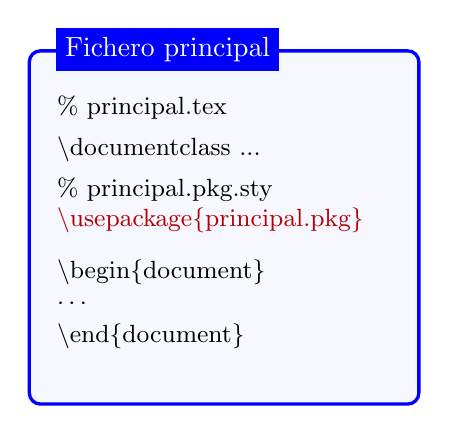
\begin{tikzpicture}
  % Define box and box title style
  \tikzstyle{myboxfichero} = [draw=blue, fill=blue!3, very thick,
  rectangle, rounded corners, inner sep=10pt, inner ysep=20pt]
  \tikzstyle{fancytitle} =[fill=blue, text=white]
    
  \node [myboxfichero] (box){%
    \begin{minipage}{0.35\textwidth}
      {\small
        
        \vspace{-1ex}
        \% principal.tex
        
        \vspace{1ex}
        
        \textbackslash documentclass ...
        
        \vspace{1ex}
        
        \% principal.pkg.sty
        
        \textcolor{red!70!black}{\textbackslash usepackage\{principal.pkg\}}
        
        \vspace{2ex}
        
        \textbackslash begin\{document\}
        
        $\cdots$
        
        \textbackslash end\{document\}
      }
    \end{minipage}
  };

  \node[fancytitle, right=10pt] at (box.north west) {Fichero principal};
  % \node[fancytitle, rounded corners] at (box.east) {$\clubsuit$};
\end{tikzpicture}%
%
\hspace{1em}
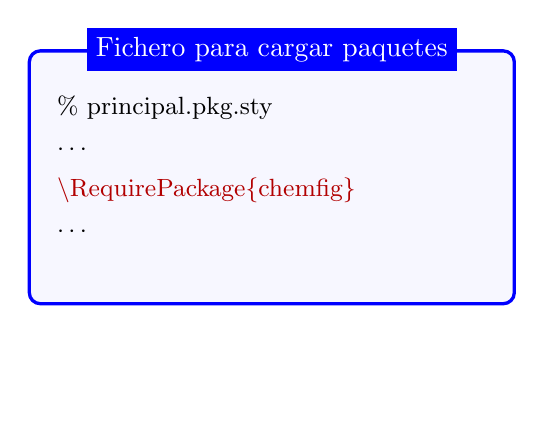
\begin{tikzpicture}[transform shape, rotate=0, baseline=-2.9cm]
  % Define box and box title style
  \tikzstyle{myboxfichero} = [draw=blue, fill=blue!3, very thick,
  rectangle, rounded corners, inner sep=10pt, inner ysep=20pt]
  \tikzstyle{fancytitle} =[fill=blue, text=white]
  
  \node [myboxfichero] (box) {%
    \begin{minipage}[t!]{0.45\textwidth}
      {\small
        \vspace{-1ex}
        \% principal.pkg.sty
        
        \vspace{1ex}
        
        $\cdots$
        \vspace{1ex}
        
        \textcolor{red!70!black}{\textbackslash RequirePackage\{chemfig\}}
        \vspace{1ex}
        
        $\cdots$
        
        \vspace{1ex}
      }
    \end{minipage}
  };
  \node[fancytitle] at (box.north) {Fichero para cargar paquetes};
\end{tikzpicture}
%

\subsection{Uso de \textsf{chemfig}}
El comando básico es \texttt{\textbackslash chemfig\{...\}}.
Su uso genérico es:
\begin{center}
\texttt{\textbackslash chemfig[lista de <claves>=<valores>]\{<código de la molécula>\}}
\end{center}

Antes de seguir mostramos una tabla con las diferentes claves, sus valores por defecto y
significado:
\begin{center}
  \begin{longtable}{rcl}\hline
    \label{tbl:chemfig_claves}
  \texttt{<clave>} & \texttt{Por defecto} & \texttt{Descripción}\\\hline
  \textcolor{blue}{\texttt{chemfig style}}
  & ---
  & Estilo que se le pasa a \texttt{tikz}\\
  \textcolor{blue}{use atom strut}
  & false
  & Tener en cuenta la caja de un átomo al situar\\&& la del siguiente\\
  \textcolor{blue}{atom style}
  & ---
  & Estilo de los nodos \emph{tikz} de los átomos\\
  \textcolor{blue}{bond join}
  & false
  & Une enlaces de forma precisa\\
  \textcolor{blue}{fixed length}
  & false
  & Todos los enlaces tienen la misma longitud\\
  \textcolor{blue}{cram rectangle}
  & false
  & No respeta el enlace triangular entre átomos\\
  \textcolor{blue}{cram width}
  & 1.5ex
  & Anchura de la base del enlace \emph{cram}\\
  \textcolor{blue}{cram dash width}
  & 1pt
  & Grosor de cada guión que forma el enlace \emph{cram}\\
  \textcolor{blue}{cram dash sep}
  & 2pt
  & Espacio entre guiones del enlace \emph{cram}\\
  \textcolor{blue}{atom sep}
  & 3em
  & Separación entre átomos\\
  \textcolor{blue}{bond offset}
  & 2pt
  & Espacio entre átomo y enlace\\
  \textcolor{blue}{double bond sep}
  & 2pt
  & Espacio entre líneas en enlaces múltiples\\
  \textcolor{blue}{angle increment}
  & 45
  & Incremento de ángulo cuando se usa código\\
  \textcolor{blue}{node style}
  & ---
  & Estilo de átomos\\
  \textcolor{blue}{bond style}
  & ---
  & Estilo de enlaces\\
  \textcolor{blue}{baseline}
  & 0pt
  & Se elige el átomo que define la altura base\\
  \textcolor{blue}{debug}
  & false
  & Muestra líneas y cajas en la fórmula\\
  \textcolor{blue}{cycle radius coeff}
  & 0.75
  & Controla tamaño del círculo aromático\\
  \textcolor{blue}{stack sep}
  & 1.5pt
  & Espaciado vertical entre argumentos de las\\&& macros \texttt{\textbackslash chemabove} y \texttt{\textbackslash chembelow}\\
  \textcolor{blue}{show cntcycle}
  & false
  & Muestra numeración en los ciclos\\
  \textcolor{blue}{autoreset cntcycle}
  & true
  & Reinicia numeración en \texttt{\textbackslash chemfigexecution}\\
  \textcolor{blue}{gchemname}
  & true
  & Utiliza las asignaciones de profundidad en \\&& \texttt{\textbackslash chemnameinit} y \texttt{\textbackslash chemnameglobal}\\
    \hline
    \caption{Tabla de claves del comando \texttt{\backslash config}.}
  \end{longtable}
\end{center}

Estas claves se muestran aquí como referencia. Las más importantes se discutirán en las
siguientes secciones.

A veces queremos modificar una opción por defecto para todo el documento, y otras
solo queremos que afecte a una fórmula o grupo de ellas:
\begin{itemize}
\item Para modificar el valor de una clave para todo el documento, podemos
  escribir en el prólogo del documento:
  \begin{center}
    \texttt{\textbackslash setchemfig\{clave=valor\}}
  \end{center}
  \item Para modificar el valor y que afecte a una fórmula, escribiríamos:
    \begin{center}
      \texttt{\textbackslash chemfig[clave=valor]\{... fórmula ...\}}
    \end{center}
\end{itemize}

Puede ser que alguna de las opciones que \textsf{chemfig} nos ofrece por defecto, por
ejemplo, la separación entre los átomos y longitud de los enlaces que nos parecieran
desproporcionadas (véase la tercera celda de la tabla de ejemplos de la sección
siguiente). En ese caso, deberíamos poder modificar esas opciones.

En ese supuesto, sería práctico poner otros valores por defecto que nos parecieran
razonables en el prólogo para todo el documento, y si quisiéramos personalizar alguna fórmula en particular dentro de este, podríamos asignar un valor concreto en ese caso,
sin afectar al resto de fórmulas.

\section{Fórmulas sencillas}
Para las fórmulas (y las reacciones químicas) sencillas se recomienda el paquete
\textsf{mhchem}, que es más fácil de utilizar.
Como primer ejemplo, veamos la fórmula molecular de un alcano:

\vspace{1ex}
\begin{tabular}{|c|}\hline
  \phantom{$\dfrac{1}{1}$} 
  \chemfig{C_nH_{2n+2}}\\
  \texttt{\textbackslash chemfig\{C\_nH\_(2n+2)\}}\\\hline
\end{tabular}

\vspace{2ex}
 Otras fórmulas:

\vspace{1ex}
\begin{tabular}{|c|c|c|c|}\hline
  \phantom{$\dfrac{1}{1}$} 
  \chemfig{NH_3}
  & \ce{H2}
  & \chemfig{CH_2=CH_2}
  & \ce{CH2=CH2}\\
  \texttt{\textbackslash chemfig\{NH\_3\}}
  & \texttt{\textbackslash ce\{H2\}}                
  & \texttt{\textbackslash chemfig\{CH\_2=CH\_2\}}
  &\texttt{\textbackslash ce\{CH2=CH2\}}\\\hline
\end{tabular}

\vspace{2ex}
 ¿Se podría arreglar la fórmula del eteno en \textsf{chemfig}? Sí, pero es menos
práctico:

\vspace{1ex}
\begin{tabular}{|c|c|}\hline
  \phantom{$\dfrac{1}{1}$} 
  \chemfig[atom sep=1.8em]{CH_2=CH_2}
  & \ce{CH2=CH2}\\
  \texttt{\textbackslash chemfig[atom sep=1.8em]\{CH\_2=CH\_2\}}
  &\texttt{\textbackslash ce\{CH2=CH2\}}\\\hline
\end{tabular}

\vspace{1ex}
 Como se puede observar, cuesta más trabajo, aunque se puede ajustar mejor la
distancia entre los átomos y por tanto, la longitud del enlace;
en este ejemplo vemos una clave de la tabla \ref{tbl:chemfig_claves}, que especifica
la distancia entre los \emph{átomos} que forman la tabla:
\begin{center}
  \texttt{atom sep=1.8em}
\end{center}
que se reducimos a casi la mitad de su valor por defecto \texttt{3em} y, como
consecuencia, el doble enlace disminuye de tamaño.

\subsection{Estado de agregación}
Se puede añadir el estado de agregación fuera del comando porque
\textsf{chemfig} solo considera los elementos que forman la sustancia, y el estado de
agregación no da esa información (aunque sí de cómo están agregados). Aquí, de nuevo es
preferible utilizar el paquete \textsf{mhchem}:

\vspace{1ex}
\begin{tabular}{|c|c|c|}\hline
  \phantom{$\dfrac{1}{1}$}
  \chemfig{Ca}(s)
  & \ce{H2O(l)}
  & \ce{He(g)}\\
  \texttt{\textbackslash chemfig\{Ca(s)\}}(s)
  & \texttt{\textbackslash ce\{H2O\}(l)}
  & \texttt{\textbackslash ce\{He(g)\}}\\\hline
\end{tabular}

\subsection{Sales con paréntesis}
\vspace{1ex}
\begin{tabular}{|c|c|}\hline
  \phantom{$\dfrac{1}{1}$}
  \chemfig{Ca{(NO_3)}_2}
  & \chemfig{{(NH4)}_2SO_3}\\
  \texttt{\textbackslash chemfig\{Ca\{(NO\_3)\}\_2\}}(s)
  & \texttt{\textbackslash chemfig\{\{(NH\_4)\}\_2SO\_3\}}\\\hline
\end{tabular}

\vspace{1ex}
 En \textsf{chemfig} es necesario encerrar los paréntesis entre llaves, pues
de lo contrario, considera que estos indican una ramificación de enlaces (que veremos
en otro momento).

\subsection{Iones}
 Los iones sencillos conviene escribirlos con \textsf{mhchem}, aunque no es
necesario:

\vspace{1ex}
\begin{tabular}{|c|c|}\hline
  \phantom{$\dfrac{1}{1}$}
  \chemfig{NO_2^{-}} & \chemfig{{NO_2}^+}\\
  \texttt{\textbackslash chemfig\{NO\_2\textasciicircum \{-\}\}}
  & \texttt{\textbackslash chemfig\{NO\_2\textasciicircum +\}}\\\hline
\end{tabular}

\vspace{1ex}
En la primera fórmula, la carga negativa se interpreta por defecto como un enlace
sencillo, por eso hay que encerrarla entre llaves; en cambio no hay problema con
la carga positiva.

Más ejemplos:

%\vspace{1ex}
\begin{tabular}{|c|c|c|}\hline
  \phantom{$\dfrac{1}{1}$}
  \chemfig{NO_3^{-}}
  & \chemfig{{NO_3}^{-}}
  & \ce{NO3-}\\
  \texttt{\textbackslash chemfig\{NO\_3\textasciicircum\{-\}\}}
  & \texttt{\textbackslash chemfig\{\{NO\_3\}\textasciicircum\{-\}\}}
  & \texttt{\textbackslash ce\{NO3-\}}\\\hline
\end{tabular}

\vspace{1ex}
 La primera fórmula no sigue las indicaciones de la IUPAC porque la carga se
sitúa justo encima del subíndice. Para solucionarla encerramos todo el grupo atómico
\ce{NO3} entre llaves.
La solución de añadir un espacio corto \texttt{\textbackslash ,} entre el subíndice
y la carga funcionaría, pero la posición de la carga variaría con el tipo de letra
que se utilice, por eso no la mostramos aquí.


\subsection{Más compuestos orgánicos sencillos}
 Veamos hidrocarburos de cadena lineal, comparando con \textsf{mhchem}:

\vspace{1ex}
\begin{tabular}{|c|c|}\hline
  \phantom{$\dfrac{1}{1}$}
  \chemfig[atom sep=1em, fixed length=true]{CH_2=CH-CH_3}
  & \ce{CH2=CH-CH3}\\
  \texttt{\textbackslash chemfig\{CH\_2=CH-CH\_3\}}
  & \texttt{\textbackslash ce\{CH2=CH-CH3\}}\\
  \texttt{[atom sep=1em, fixed length=true]} & \\\hline
\end{tabular}

\vspace{1ex}
 Para acortar anchura de las primera celda de izquierda de la tabla, hemos
separado las claves del comando \texttt{\textbackslash chemfig}. El comando completo
sería:
\begin{center}
  \texttt{%
    \textbackslash chemfig[atom sep=1em,fixed length=true]\{CH\_2=CH-CH\_3\}
  }
\end{center}


\vspace{1ex}
\begin{tabular}{|c|c|}\hline
  \phantom{$\dfrac{1}{1}$}
  \chemfig[atom sep=1em, fixed length=true]{CHOH=CH-CH_2Cl}
  & \ce{CHOH=CH-CH2Cl}\\
  \texttt{\textbackslash chemfig\{CHOH=CH-CH\_2Cl\}}
  & \texttt{\textbackslash ce\{CHOH=CH-CH\_2Cl\}}\\
  \texttt{[atom sep=1em, fixed length=true]} & \\\hline
\end{tabular}


\vspace{1ex}
 Aquí hemos utilizado otra clave de la tabla \ref{tbl:chemfig_claves}:
\begin{center}
  \texttt{fixed length=true}
\end{center}
que obliga a utilizar la misma longitud para todos los enlaces en la fórmula.

\vspace{1ex}
\begin{tabular}{|c|c|}\hline
  \phantom{$\dfrac{1}{1}$}
  \chemfig[atom sep=1em, fixed length=true]{CH_3-{(CH_2)}_n-CH_3}
  & \ce{CH3-(CH2)_n-CH3}\\
  \texttt{\textbackslash chemfig\{CH\_3-\{(CH\_2)\}\_n\}-CH\_3}
  & \texttt{\textbackslash ce\{CH3-(CH2)\_n-CH3\}}\\
  \texttt{[atom sep=1em, fixed length=true]} & \\\hline
\end{tabular}

\vspace{2ex}
La razón  de tener que encerrar el paréntesis entre llaves de debe a la forma particular
con que \textsf{chemfig} trata los elementos de una fórmula. Aunque lo veremos con más
detalle más tarde, \textsf{chemfig} considera que esta fórmula está formada por tres
\emph{grupos de átomos}: "\ce{CH3}", "\ce{(CH2)_n}" y "\ce{CH3}".

Después considera que el primer y el tercer grupo está formado por dos \emph{átomos},
"\ce{C}" y "\ce{H3}", pero el segundo grupo no está formado por \emph{átomos}, porque
\textsf{chemfig} no contempla la posibilidad de paréntesis, de hecho, el paréntesis se
interpreta como una ramificación de enlaces y, para desactivarla hay que encerrar los
paréntesis entre llaves.


\vspace{2ex}
Los enlaces triples se representan con la tilde, \texttt{\textasciitilde}:

\vspace{1ex}
\begin{tabular}{|c|c|}\hline
  \phantom{$\dfrac{1}{1}$}
  \chemfig[atom sep=1.5em]{CH~CH}
  & \ce{CH#CH}\\
  \texttt{\textbackslash chemfig\{CH\textasciitilde CH\}}
  & \texttt{\textbackslash ce\{CH\#CH\}}\\
  \texttt{[atom sep=1.5em]} & \\\hline
\end{tabular}



\section{Enlaces químicos}
Los enlaces (junto con los elementos) son el foco de la formulación. No es de
extrañar que \textsf{chemfig}, permita configurarlos de muchas maneras. Así, dejamos
en parte la escritura de fórmulas concretas (no del todo) y nos esforzaremos en explicar
los detalles más importantes.

\subsection{Tipos de enlace}

En \textsf{chemfig} hay nueve tipos de enlace:
\begin{center}
  {\normalsize
  \begin{longtable}{lrcl}\hline
    \label{tbl:chemfig_enlaces}
   \texttt{\#} & \texttt{Código} & \texttt{Resultado} & \texttt{Tipo de enlace}\\\hline
    1
    & \textcolor{blue}{\texttt{\textbackslash chemfig{\{A-B\}}}}
    & \chemfig{A-B}
    & Sencillo\\
    2
    & \textcolor{blue}{\texttt{\textbackslash chemfig{\{A=B\}}}}
    & \chemfig{A=B}
    & Doble\\
    3
    &\textcolor{blue}{\texttt{\textbackslash chemfig{\{A\textasciitilde B\}}}}
    & \chemfig{A~B}
    & Triple\\
    4
    & \textcolor{blue}{\texttt{\textbackslash chemfig{\{B>A\}}}}
    & \chemfig{B>A}
    & Triangular izquierdo relleno\\
    5
    & \textcolor{blue}{\texttt{\textbackslash chemfig{\{A<B\}}}}
    & \chemfig{A<B}
    & Triangular derecho relleno\\
    6
    & \textcolor{blue}{\texttt{\textbackslash chemfig{\{B>:A\}}}}
    & \chemfig{B>:A}
    & Triangular izquierdo rayado\\
    7
    & \textcolor{blue}{\texttt{\textbackslash chemfig{\{A<:B\}}}}
    & \chemfig{A<:B}
    & Triangular derecho rayado\\
    8
    & \textcolor{blue}{\texttt{\textbackslash chemfig{\{A<|B\}}}}
    & \chemfig{A<|B}
    & Triangular derecho hueco\\
    9
    & \textcolor{blue}{\texttt{\textbackslash chemfig{\{B>|A\}}}}
    & \chemfig{B>|A}
    & Triangular izquierdo hueco\\
    \hline
    \caption{Enlaces en \textsf{chemfig}.}
  \end{longtable}
  }
\end{center}

\subsection{\texttt{double bond sep}}
 La clave
\begin{center}
  \texttt{double bond sep=<dim>}
\end{center}
indica la separación entre las líneas que forman los
enlaces múltiples (doble y triple); \texttt{<dim>} es una dimensión, que por defecto es
de $2pt$.
Ejemplos:

\vspace{1ex}
\begin{tabular}{|c|c|}\hline
  \phantom{$\dfrac{1}{1}$}
  \chemfig[atom sep=1.5em]{CH~CH}
  & \chemfig[atom sep=1.5em,double bond sep=1.2pt]{CH~CH}\\
  \texttt{\textbackslash chemfig\{CH\textasciitilde CH\}}
  & \texttt{\textbackslash chemfig\{CH\textasciitilde CH\}}\\
  \texttt{[atom sep=1.5em]} & \texttt{[atom sep=1.5em,double bond sep=1.5pt]}\\\hline
\end{tabular}

\subsection{\texttt{double bond sep}, \texttt{atom sep}, \texttt{bond offset} y \texttt{bond style}}

\vspace{1ex}
Cuando se sitúa un enlace entre dos átomos hay varios aspectos a considerar:
\begin{itemize}
\item El primero es que cada \emph{átomo} (que puede ser \ce{C}, \ce{Cl}, \ce{CH2}, etc.),
  se encierra en una caja (\emph{bounding box}). En la figura que sigue son los puntos
  rojos en el centro de las cajas.
\item El segundo es la distancia $\Delta$ entre los centros de las cajas, que se
  configura mediante \texttt{atom sep}.
\item El tercero es la distancia $\delta$ entre el borde una caja y el lugar donde
  comienza a dibujarse el enlace, que se configura mediante \texttt{bond offset}.
\end{itemize}

\begin{center}
  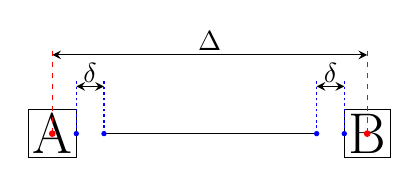
\begin{tikzpicture}[%
    every node/.style={%
      anchor=base,inner sep=1.5pt,outer sep=0pt,minimum size=0pt},
    baseline
    ]
    \node[draw] at(0,0)(aa){\huge A};
    \node[draw]at(4,0)(bb){\huge B};
    \path[shorten <=10pt,shorten >=10pt,draw]
    (aa)--(bb)coordinate[pos=0](al) coordinate[pos=1](bl);
    \node[draw,circle,fill,blue,minimum size=1.5pt,inner sep=0pt]at(al){};
    \node[draw,circle,fill,blue,minimum size=1.5pt,inner sep=0pt]at([xshift=10pt]al){};
    \node[draw,circle,fill,blue,minimum size=1.5pt,inner sep=0pt]at(bl){};
    \node[draw,circle,fill,blue,minimum size=1.5pt,inner sep=0pt]at([xshift=-10pt]bl){};
    \draw[blue,dash pattern=on 1pt off 1pt](bl)--([yshift=0.7cm]bl);
    \draw[blue,dash pattern=on 1pt off 1pt]
    ([xshift=-10pt]bl)--([xshift=-10pt,yshift=0.7cm]bl);
    \draw[stealth-stealth]
    ([yshift=0.6cm]bl.center)--([xshift=-10pt,yshift=0.6cm]bl.center)
    node [midway,above,draw=none]{$\delta$};
    \draw[blue,dash pattern=on 1pt off 1pt](al)--([yshift=0.7cm]al);
    \draw[blue,dash pattern=on 1pt off 1pt]
    ([xshift=10pt]al)--([xshift=10pt,yshift=0.7cm]al);
    \draw[stealth-stealth]
    ([yshift=0.6cm]al.center)--([xshift=10pt,yshift=0.6cm]al.center)
    node [midway,above,draw=none]{$\delta$};
    \node[draw,circle,fill,red,minimum size=2pt,inner sep=0pt]at(aa){};
    \node[draw,circle,fill,red,minimum size=2pt,inner sep=0pt]at(bb){};
    \draw[stealth-stealth]
    ([yshift=1cm]aa.center)--([yshift=1cm]bb.center)
    node [midway,above,draw=none] {$\Delta$};
    \draw[red,dash pattern=on 2pt off2pt](aa.center)--([yshift=1.1cm]aa.center);
    \draw[red,dash pattern=on 2pt off2pt](bb.center)--([yshift=1.1cm]bb.center);
  \end{tikzpicture}
\end{center}

\vspace{2ex}
Estudiaremos tres claves del comando \texttt{\textbackslash chemfig}, relacionadas con
los enlaces:
\begin{itemize}
\item \texttt{atom sep}:

Separación entre los centros de las cajas de los átomos.
  
\begin{tabular}{|c|c|}\hline
  \phantom{$\dfrac{1}{1}$}
  \chemfig[atom sep=2em]{A-B}
  & \chemfig[atom sep=50pt]{A-B}\\
  \texttt{\textbackslash chemfig\{A-B\}}
  & \texttt{\textbackslash chemfig\{A-B\}}\\
  \texttt{[atom sep=2em]} & \texttt{[atom sep=50pt]}\\\hline
\end{tabular}
\item \texttt{bond offset}:

Separación entre borde de caja de átomo y principio del dibujo del enlace.
  
\begin{tabular}{|c|c|}\hline
  \phantom{$\dfrac{1}{1}$}
  \chemfig[bond offset=0pt]{A-B}
  & \chemfig[bond offset=5pt]{A-B}\\
  \texttt{\textbackslash chemfig\{A-B\}}
  & \texttt{\textbackslash chemfig\{A-B\}}\\
  \texttt{[bond offset=0pt]} & \texttt{[bond offset=5pt]}\\\hline
\end{tabular}

Si queremos aplicar un espacio de separación diferente para un enlace determinado
en una fórmula, se puede añadir \texttt{\#} justo después del enlace.
En el ejemplo suponemos que por defecto hemos establecido para todos los enlaces
una distancia entre átomo y enlace un espaciado de $6pt$ (en realidad, entre el
extremo de la caja y el comienzo del enlace). En la primera fórmula indicamos que
el primer enlace tiene un espaciado de $0pt$ al principio. En la segunda especificamos
que el segundo enlace tenga un espaciado de $2pt$ al final de este. En la tercera
dejamos el espaciado por defecto.

{%
  \setchemfig{bond offset=8pt}
  \begin{tabular}{|c|c|c|}\hline
    \multicolumn{3}{|c|}{%
    {\large\texttt{\textbackslash setchemfig\{bond offset=6pt\}}}
    }\\\hline
    \phantom{$\dfrac{1}{1}$}
    \chemfig{A-#(0pt,0pt)B-C}
    & \chemfig{A-B-#(,2pt)C}
    & \chemfig{A-B-#(2pt)C}\\
    \texttt{\textbackslash chemfig\{A-B\}}
    & \texttt{\textbackslash chemfig\{A-B\}}
    & \texttt{\textbackslash chemfig\{A-B\}}\\
    \texttt{[bond offset=0pt]}
    & \texttt{[bond offset=0pt]}    
    & \texttt{[bond offset=5pt]}\\\hline
  \end{tabular}
}


\item \texttt{bond style}:
  
  A los enlaces de la fórmula se le aplican los estilos del paquete de dibujo
  \textsf{tikz}.

\begin{tabular}{|c|c|}\hline
  \phantom{$\dfrac{1}{1}$}
  \chemfig[bond style={line width=1pt,red}]{A>|B=C-D<:E}
  & \chemfig[bond style={line width=1pt,dotted,red}]{A-B}\\
  \texttt{\textbackslash chemfig\{A>|B=C-D<:E\}}
  & \texttt{\textbackslash chemfig\{A-B\}}\\
  {\footnotesize\texttt{[bond style=\{line width=1pt,red\}]}}
  & {\footnotesize\texttt{[bond style=\{line width=1pt,dotted,red\}]}}\\
  \hline
\end{tabular}
\end{itemize}

\subsection{Ángulos en los enlaces}
Hasta ahora hemos dibujado los enlaces horizontalmente, formando un ángulo de
\qty{0}{\degree} medido desde el átomo de partida. Si no se especifica nada, este
es el ángulo por defecto, pero podemos cambiarlo.

Hay varias formas de especificar los ángulos. Se pueden utilizar todas en una fórmula:
\begin{itemize}
\item Múltiplos de \qty{45}{\degree}:

  En este caso, este indica el múltiplo de \qty{45}{\degree} que forma el ángulo con
  respecto del átomo de partida. Este número se escribe entre corchetes:

  % \vspace{1ex}
\begin{tabular}{|c|c|c|c|}\hline
  \phantom{\rule{0.4pt}{10ex}}
  \chemfig{A-B}
  & \chemfig{A-[1]B}
  & \chemfig{A-[2]B}
  & \chemfig{A-[3]B}\\
  {\footnotesize\texttt{\textbackslash chemfig\{A-B\}}}
  & {\footnotesize\texttt{\textbackslash chemfig\{A-[1]B\}}}
  & {\footnotesize\texttt{\textbackslash chemfig\{A-[2]B\}}}
  & {\footnotesize\texttt{\textbackslash chemfig\{A-[3]B\}}}\\
  \qty{0}{\degree}
  & \qty{45}{\degree}
  & \qty{90}{\degree}
  & \qty{135}{\degree}
  \\\hline
\end{tabular}

\begin{tabular}{|c|c|c|c|}\hline
  \phantom{\rule{0.4pt}{3ex}}
  \chemfig{A-[4]B}
  & \chemfig{A-[5]B}
  & \chemfig{A-[6]B}
  & \chemfig{A-[7]B}\\
  {\footnotesize\texttt{\textbackslash chemfig\{A-[4]B\}}}
  & {\footnotesize\texttt{\textbackslash chemfig\{A-[5]B\}}}
  & {\footnotesize\texttt{\textbackslash chemfig\{A-[6]B\}}}
  & {\footnotesize\texttt{\textbackslash chemfig\{A-[7]B\}}}\\
  \qty{180}{\degree}
  & \qty{-135}{\degree}
  & \qty{-90}{\degree}
  & \qty{-45}{\degree}
  \\\hline
\end{tabular}

\item Ángulos absolutos:

  El ángulo absoluto se escribe entre corchetes precedido de dos puntos:
  Ejemplos:

  % \vspace{1ex}
\begin{tabular}{|c|c|}\hline
  \phantom{\rule{0.4pt}{5ex}}
  \chemfig{A-B-[:-45]C-D-[:90]E}
  & \chemfig[atom sep=2em]{-[:30]-[:-30]-[:-90]-[:-150]-[:150]-[:90]}\\
  {\scriptsize\texttt{\textbackslash chemfig\{A-B-[:-45]C-D-[:90]E\}}}
  & {\scriptsize\texttt{\textbackslash chemfig\{-[:30]-[:-30]-[:-90]-[:-150]-[:150]-[:90]\}}}\\
  & \texttt{[atom sep=2em]}
  \\\hline
\end{tabular}

\item Ángulos relativos:

  El ángulo relativo, con respecto al anterior, se escribe entre corchetes precedido de doble carácter de dos puntos:
  Ejemplos:

  % \vspace{1ex}
  \begin{tabular}{|c|c|}\hline
    \phantom{\rule{0.4pt}{8ex}}
    \chemfig{A-B-[::45]C=[::-60]D}
    & \chemfig{-[:36]-[::-72]-[::-72]-[::-72]-[::-72]}\\
    {\scriptsize\texttt{\textbackslash chemfig\{A-B-[::45]C=[::-60]D\}}}
    & {\scriptsize\texttt{\textbackslash chemfig\{-[:-36]-[:-72]-[::-72]-[:-72]-[:-72]\}}}
    \\\hline
  \end{tabular}
\end{itemize}

\subsection{Longitud de los enlaces}
Por lo visto hasta ahora, en lugar de longitud de enlace deberíamos hablar de espaciado
interatómico (\texttt{atom sep}). Este espaciado se tiene en cuenta cuando
\texttt{fixed length=false}, que está por defecto. De esta manera \textsf{chemfig}
utiliza un espaciado interatómico fijo:

\begin{center}
\begin{tabular}{c@{\kern2cm}c}
	\CFkv{fixed length}{false}&\CFkv{fixed length}{true}\\[2ex]
  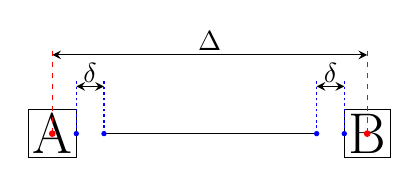
\begin{tikzpicture}[%
    every node/.style={anchor=base,inner sep=1.5pt,outer sep=0pt, minimum size=0pt},
    baseline
    ]
	\node[draw] at(0,0)(aa){\huge A};
	\node[draw]at(4,0)(bb){\huge B};
	\path[shorten <=10pt,shorten >=10pt,draw]
        (aa)--(bb)coordinate[pos=0](al) coordinate[pos=1](bl);
	\node[draw,circle,fill,blue,minimum size=1.5pt,inner sep=0pt]at(al){};
	\node[draw,circle,fill,blue,minimum size=1.5pt,inner sep=0pt]
        at([xshift=10pt]al){};
	\node[draw,circle,fill,blue,minimum size=1.5pt,inner sep=0pt]at(bl){};
	\node[draw,circle,fill,blue,minimum size=1.5pt,inner sep=0pt]
        at([xshift=-10pt]bl){};
	\draw[blue,dash pattern=on 1pt off 1pt](bl)--([yshift=0.7cm]bl);
	\draw[blue,dash pattern=on 1pt off 1pt]
        ([xshift=-10pt]bl)--([xshift=-10pt,yshift=0.7cm]bl);
	\draw[stealth-stealth]
        ([yshift=0.6cm]bl.center)--([xshift=-10pt,yshift=0.6cm]bl.center)
        node [midway,above,draw=none]{$\delta$};
	\draw[blue,dash pattern=on 1pt off 1pt](al)--([yshift=0.7cm]al);
	\draw[blue,dash pattern=on 1pt off 1pt]
        ([xshift=10pt]al)--([xshift=10pt,yshift=0.7cm]al);
	\draw[stealth-stealth]
        ([yshift=0.6cm]al.center)--([xshift=10pt,yshift=0.6cm]al.center)
        node [midway,above,draw=none]{$\delta$};
	\node[draw,circle,fill,red,minimum size=2pt,inner sep=0pt]at(aa){};
	\node[draw,circle,fill,red,minimum size=2pt,inner sep=0pt]at(bb){};
	\draw[stealth-stealth]
        ([yshift=1cm]aa.center)--([yshift=1cm]bb.center)
        node [midway,above,draw=none] {$\Delta$} ;
	\draw[red,dash pattern=on 2pt off2pt](aa.center)--([yshift=1.1cm]aa.center);
	\draw[red,dash pattern=on 2pt off2pt](bb.center)--([yshift=1.1cm]bb.center);
      \end{tikzpicture}
      &
      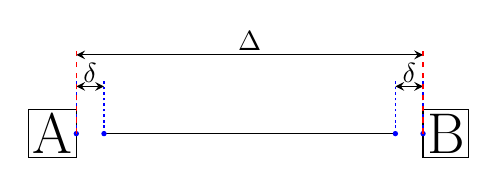
\begin{tikzpicture}[%
        every node/.style={anchor=base,inner sep=1.5pt,outer sep=0pt,minimum size=0pt},
        baseline]
        \node[draw] at(0,0)(aa){\huge A};
        \node[draw]at(5,0)(bb){\huge B};
        \path[shorten <=10pt,shorten >=10pt,draw]
        (aa)--(bb)coordinate[pos=0](al) coordinate[pos=1](bl);
        \node[draw,circle,fill,blue,minimum size=1.5pt,inner sep=0pt]at(al){};
        \node[draw,circle,fill,blue,minimum size=1.5pt,inner sep=0pt]
        at([xshift=10pt]al){};
        \node[draw,circle,fill,blue,minimum size=1.5pt,inner sep=0pt]at(bl){};
        \node[draw,circle,fill,blue,minimum size=1.5pt,inner sep=0pt]
        at([xshift=-10pt]bl){};
	\draw[blue,dash pattern=on 1pt off 1pt](bl)--([yshift=0.7cm]bl);
	\draw[blue,dash pattern=on 1pt off 1pt]
        ([xshift=-10pt]bl)--([xshift=-10pt,yshift=0.7cm]bl);
	\draw[stealth-stealth]
        ([yshift=0.6cm]bl.center)--([xshift=-10pt,yshift=0.6cm]bl.center)
        node [midway,above,draw=none]{$\delta$};
	\draw[blue,dash pattern=on 1pt off 1pt](al)--([yshift=0.7cm]al);
	\draw[blue,dash pattern=on 1pt off 1pt]
        ([xshift=10pt]al)--([xshift=10pt,yshift=0.7cm]al);
	\draw[stealth-stealth]
        ([yshift=0.6cm]al.center)--([xshift=10pt,yshift=0.6cm]al.center)
        node [midway,above,draw=none]{$\delta$};
	\draw[stealth-stealth]([yshift=1cm]al)--([yshift=1cm]bl)
        node [midway,above,draw=none] {$\Delta$} ;
	\draw[red,dash pattern=on 2pt off2pt](al)--([yshift=1.1cm]al);
	\draw[red,dash pattern=on 2pt off2pt](bl)--([yshift=1.1cm]bl);
      \end{tikzpicture}
  \end{tabular}
\end{center}

En el siguiente ejemplo, los átomos en la molécula de yodo entre sí y los del \ce{H3} con
el \ce{C} están situados a la misma distancia y, como consecuencia, la longitud de enlace
es diferente:

\begin{tabular}{|c|c|}\hline
  \phantom{\rule{0.4pt}{2.5ex}}
  \chemfig{I-I}
  & \chemfig{CH_3-CH_3}\\
  \texttt{\textbackslash chemfig\{I-I\}}
  & \texttt{\textbackslash chemfig\{CH\_3-CH\_3\}}\\\hline
\end{tabular}

\vspace{1ex}
Comparamos el resultado de los comandos anteriores:
\begin{center}
\begin{tabular}{|c|}\hline
  \chemfig{I-I}\\
  \chemfig{CH_3-CH_3}\\\hline
\end{tabular}
\end{center}

Pero, cuando indicamos \texttt{fixed length=true}, la longitud de enlace es relativamente
constante, aunque depende además, de la inclinación del enlace y del tamaño del átomo.
Para la longitud del enlace se toma la distancia definida en \texttt{atom sep=<dim>}:
Veamos un ejemplo:
\begin{center}
\begin{tabular}{|c|}\hline
  \chemfig[fixed length=true]{I-I}\\
  \chemfig[fixed length=true]{CH_3-CH_3}\\\hline
\end{tabular}
\end{center}

Incluso así, cuando los átomos con \texttt{fixed length=true}, se encuentran en un
ciclo, no se respeta tal condición, sino que se da prioridad a la distancia
interatómica constante, para que el ciclo sea regular.

En algunas situaciones, especialmente, cuando \textsf{chemfig} tiene el comportamiento
por defecto (\texttt{fixed length=false}), pueden formarse enlaces muy cortos y se
necesitaría aumentar (o disminuir) la distancia interatómica en algún enlace concreto.
Para ello, no vale \texttt{\textbackslash chemfig[atom sep=valor]\{...\}}, porque
afectaría a todos los enlaces de la molécula.

Se puede indicar esa distancia en un enlace concreto añadiendo argumentos entre
corchetes. Ya vimos que el primer argumento indicaba el ángulo que formaba el enlace.
Un segundo argumento, separado del primero por una coma, indica la distancia
interatómica. Ejemplo:

\begin{tabular}{|c|c|}\hline
  \phantom{\rule{0.4pt}{3ex}}
  \chemfig{{A_2}^{2+}-B_3}
  & \chemfig{{A_2}^{2+}-[,2]B_3}\\
  \texttt{%
  \textbackslash chemfig\{\{A\_2\}\textasciicircum\{2+\}-B\_3\}
  }
  & \texttt{%
    \textbackslash chemfig\{%
    \{A\_2\}\textasciicircum\{2+\}-[,2]B\_3\}}\\\hline
\end{tabular}

En el ejemplo de la derecha, el enlace sencillo viene acompañado del corchete
\texttt{[,2]}. El primer argumento está vacío, por lo que se utilizará para el enlace el
ángulo por defecto, \qty{0}{\degree}. El segundo argumento es un $2$, lo que indica que la
distancia interatómica para ese enlace es el doble de la especificada en
\texttt{atom sep}.


Podemos cambiar el tamaño de las moléculas cambiando el tamaño de la fuente, los
enlaces se escalan de forma apropiada si \texttt{atom sep} se ha definido en función
de la fuente, por ejemplo \text{em} o \text{ex}. Porque estas unidades dependen de
la fuente elegida.

\begin{tabular}{|c|c|}\hline
  \phantom{\rule{0.4pt}{7ex}}
  \chemfig{H-[:37]O-[::-72]H}
  & {\small\chemfig{H-[:37]O-[::-72]H}}\\
  \texttt{\{\textbackslash chemfig\{H-[:37]O-[::-72]H\}\}}
  & \texttt{\{\textbackslash small
    \!\!\!\!\textbackslash chemfig\{H-[:37]O-[::-72]H\}\}}\\\hline
\end{tabular}


\subsection{Átomos de salida y llegada}
Un grupo de átomos suele estar formado por varios átomos, como \ce{CH3}, que está
formado por los \emph{átomos} \ce{C} y \ce{H3}. Supongamos que nos interesa unir
mediante enlaces dos grupos de átomos, digamos \ce{ABCD} y \ce{EFG}. Por defecto,
\textsf{chemfig} intentará unir los átomos que tenga más cerca dependiendo del ángulo que
se especifique:

{\small
\begin{tabular}{|c|c|c|}\hline
  \phantom{\rule{0.4pt}{6ex}}
  \chemfig{ABC-DEF}
  & \chemfig{ABC-[:30]DEF}
  & \chemfig{ABC-[:150]DEF}\\
  \texttt{\{\textbackslash chemfig\{ABC-DEF\}\}}
  &\texttt{\{\textbackslash chemfig\{ABC-[:30]DEF\}\}}
  & \texttt{\textbackslash chemfig\{ABC-[:150]DEF\}\}}\\\hline
\end{tabular}
}

¿Cómo podríamos obligar a \textsf{chemfig} a unir átomos distintos a los que elige?
Ya hemos visto dos argumentos a cada enlace particular, el primero era el ángulo del
enlace, el segundo es la separación de los átomos, el tercero indica el átomo desde
el que sale el enlace y el cuarto el átomo al que llega:
\begin{center}
  {\small
    \texttt{"enlace"%
      [ángulo,distancia entre átomos,\textbf{átomo de salida},\textbf{átomo de llegada]}
    }
  }
\end{center}
Los átomos de salida y llegada se indican mediante números naturales.
Veamos dos ejemplos:

\begin{tabular}{|c|c|}\hline
  \phantom{\rule{0.4pt}{10ex}}
  \chemfig{ABC-[:80,,1,1]DEF}
  & \chemfig{ABC-[:90,,2,1]DEF}\\
  \texttt{\{\textbackslash chemfig\{ABC-[:80,,1,1]DEF\}\}}
  & \texttt{\textbackslash chemfig\{ABC-[:90,,2,1]DEF\}\}}\\\hline
\end{tabular}


\subsection{Personalización mediante \textsf{tikz}}
Hay un quinto argumento para personalizar un enlace: \texttt{,,,,<tikz>}.
Veamos unos ejemplos:

\begin{tabular}{|cl|}\hline
  \phantom{\rule{0.4pt}{2ex}}
  \chemfig{A-[,,,,line width=1.4pt,red]B}
  & {\footnotesize
    \texttt{\textbackslash chemfig\{A-[,,,,line width=1.2pt,red]B\}}
    }\\\hline
  \chemfig{A-[,,,,line width=0.8pt,dash pattern=on 2pt off 2pt,blue]B}
  & {\footnotesize
    \texttt{%
    \textbackslash chemfig\{A-[,,,,line width=0.8pt,dash pattern=on 2pt off 2pt]B\}}
    }\\\hline
  \chemfig{A-[,1.5,,,decorate,decoration=snake]B}
  & {\footnotesize
    \texttt{%
    \textbackslash chemfig\{A-[,2,,,decorate,decoraton=snake]B\}}
    }\\\hline
  \chemfig{A-[,1.4,,,decorate,decoration=coil,segment length=0.3em]B}
  & {\footnotesize
    \texttt{%
    \textbackslash chemfig\{A-[,1.4,,,decorate,decoration=coil,segment length=0.3em]B\}}
    }\\\hline
\end{tabular}


\subsection{Conectando enlaces}
Cuando se unen enlaces entre sí, no se ajustan perfectamente, sobre todo esto es
visible cuando la anchura del enlace es grande. Para que se unan perfectamente hay que
añadir \texttt{bond join=true} o simplemente \texttt{bond join}. Veamos los siguientes
ejemplos:

\begin{tabular}{|cl|}\hline
  \phantom{\rule{0.4pt}{6ex}}
  \chemfig{-[:45]-[::-90]}
  & {\small
    \texttt{\textbackslash chemfig\{-[:45]-[::-90]\}}
    }\\\hline
  \phantom{\rule{0.4pt}{6ex}}
  \chemfig[bond style={line width=3.5pt}]{-[:45]-[::-90]}
  & {\small
    \texttt{%
    \textbackslash chemfig[bond style=\{line width=3.5pt\}]\{-[:45]-[::-90]\}}
    }\\\hline
  \phantom{\rule{0.4pt}{6ex}}
  \chemfig[bond join,bond style={line width=3.5pt}]{-[:45]-[::-90]}
  & {\footnotesize
    \texttt{%
    \textbackslash chemfig[bond join,bond style=\{line width=3.5pt\}]\{-[:45]-[::-90]\}}
    }\\\hline
  \phantom{\rule{0.4pt}{6ex}}
  \chemfig[bond join=true]{-[:45]-[::-90]}
  & {\small
    \texttt{\textbackslash chemfig[bond join=true]\{-[:45]-[::-90]\}}
    }\\\hline
\end{tabular}


\subsection{Valores por defecto para los enlaces}
Las propiedades de los enlaces están determinadas por cinco parámetros:
\begin{center}
  \texttt{[ángulo, coeficiente, salida, llegada, tikz]}
\end{center}

Si no se especificaran estos parámetros, \textsf{chemfig} utiliza los siguientes:
\begin{enumerate}
\item Ángulo: \qty{0}{\degree}. El enlace se dirige de izquierda a derecha.
\item Coeficiente: 1. La distancia entre los átomos o la longitud del enlace es
  1 multiplicado por la distancia especificada para \texttt{atom sep}, según sea
  el valor especificado a \texttt{fixed length}.
\item Átomos de salida y llegada: vacíos. Lo que indica que el enlace se dirige
  entre los dos átomos más cercanos, teniendo en cuenta el ángulo que forma el enlace.
\item Estilo tikz: vacío. No añade ningún estilo especial de \textsf{tikz}.
\end{enumerate}

Además, estos se pueden establecer:
\begin{itemize}
\item En el prólogo del documento, para todas las fórmulas, por defecto:
  \begin{center}
    \texttt{\textbackslash setchemfig\{ángulo,coeficiente,salida,llegada,tikz\}}
  \end{center}
\item Para una molécula en particular, al principio del comando
  \texttt{\textbackslash chemfig}, cuyo efecto . Veamos
  dos ejemplos. En el primero, especificamos un ángulo de enlace y distancia
  interatómica para el primer enlace; al segundo enlace no le afecta. En el segundo
  ejemplo, definimos color rojo al principio del comando, por lo que afectará a todos
  los enlaces, a menos que se indique otra cosa para algún o algunos enlaces en
  particular, en este ejemplo, para el doble enlace indicamos color verde y el último
  enlace vuelve a ser rojo, como habíamos indicado por defecto en esta molécula:
    
  \begin{tabular}{|cl|}\hline
    \phantom{\rule{0.4pt}{6ex}}
    \chemfig{A-[:15,2,,,,red]B-C}
    & {\small
      \texttt{\textbackslash chemfig\{A-[:15,2,,,,red]B-C\}}
      }\\\hline
    \phantom{\rule{0.4pt}{3ex}}
    \chemfig{[,,,,red]A-B-C=[,,,,green]D-E}
    & {\footnotesize
      \texttt{%
      \textbackslash chemfig\{[,,,,red]A-B-C=[,,,,green]D-E\}}
      }\\\hline
  \end{tabular}
\end{itemize}

\subsection{Ramificaciones}
Hasta ahora hemos visto moléculas que hemos escrito linealmente. Se pueden añadir
\emph{ramificaciones} a las anteriores (esto también servirá para las ramificaciones,
una vez que veamos los ciclos).

En el primer ejemplo representamos una fórmula genérica lineal \ce{A-B-C}.
En el segundo ejemplo, añadimos en el segundo átomo de la cadena, la ramificación \texttt{-[2]W-X}, que se encierra entre paréntesis (recordemos que el número 2 indica que
la ramificación forma un ángulo de $2\cdot\qty{45}{\degree}=\qty{90}{\degree}$:

\begin{tabular}{|c|c|}\hline
  \phantom{\rule{0.4pt}{10ex}}
  \chemfig{A-B-C}
  & \chemfig{A-B(-[2]W-X)-C}\\
  \texttt{%
  \textbackslash chemfig\{A-B-C\}
  }
  & \texttt{%
    \textbackslash chemfig\{%
    \{A-B(-[2]W-X)-C\}}\\\hline
\end{tabular}

Aunque la fórmula anterior se ha escrito y se lee fácilmente, suele ser recomendable
dibujar la estructura base (que no necesariamente cadena lineal) que tenga más átomos,
y el resto como ramificaciones. Por tanto la fórmula anterior se podría haber escrito
de varias formas. Una de ellas es representar la estructura base de cuatro átomos
\ce{A-B-W-X} y añadir como ramificación la \ce{C}:

\begin{tabular}{|c|c|}\hline
  \phantom{\rule{0.4pt}{10ex}}
  \chemfig{A-B-[2]W-X}
  & \chemfig{A-B(-C)-[2]W-X}\\
  \texttt{%
  \textbackslash chemfig\{A-B-[2]W-X\}
  }
  & \texttt{%
    \textbackslash chemfig\{%
    \{A-B(-C)-[2]W-X}\\\hline
\end{tabular}


\subsection{Ejemplos}
Para estos ejemplos utilizaremos unas distancias interatómicas más cortas:

\texttt{
\noindent\textbackslash setchemfig\{\\
\hspace*{2em}atom sep=2.0em, {\small\% Reduce la longitud de los enlaces}\\
\hspace*{2em}bond offset=2pt, {\small\% Espacio entre el átomo y el inicio del enlace}\\
\hspace*{2em}double bond sep=2.5pt, {\small\% Espacio entre líneas de un enlace múltiple}\\
\hspace*{2em}bond spacing=3.0pt, {\small\% Espacio reservado para los enlaces múltiples}\\
\hspace*{2em}cram size=3pt, {\small\% Ancho de la base de los enlaces de tipo Cram (cuñas)}\\
\hspace*{2em}node style=\{scale=0.85\} {\small\% Escala las etiquetas de los átomos}\\
\}}


\setchemfig{
  atom sep = 2.0em,       % Reduce la longitud de los enlaces (por defecto es 3.0em)
  bond offset = 2pt,      % Espacio entre el átomo y el inicio del enlace
  double bond sep = 2.5pt,% Espacio entre las dos líneas de un enlace doble
  bond spacing = 3.0pt,   % Espacio entre los puntos de un par solitario (Lewis)
  cram size = 3pt,        % Ancho de la base de los enlaces de tipo Cram (cuñas)
  node style = {scale=0.85} % Escala ligeramente las etiquetas de los átomos
}


Empezamos con unas cuantas versiones del \emph{isobutano}:

\begin{tabular}{|c|c|}\hline
  \phantom{\rule{0.4pt}{7ex}}
  \chemfig{CH_3-CH(-[2]CH_3)-CH_3}
  & \chemfig{CH_3-CH(-[6]CH_3)-CH_3}\\
  {\small\texttt{%
  \textbackslash chemfig\{CH\_3-CH(-[2]CH\_3)-CH\_3\}
  }}
  & {\small\texttt{%
    \textbackslash chemfig\{CH\_3-CH(-[2]CH\_3)-CH\_3\}
    }}
  \\\hline
\end{tabular}

\vspace{1ex}
A partir de ahora, siempre que sea posible evitaremos escribir el comando
\begin{center}
  \texttt{\textbackslash chemfig}
\end{center}
aunque sí las llaves que le siguen. El propósito de esto es disminuir la anchura de las
celdillas en los ejemplos. Así, en lugar de la tabla anterior, la escribiremos como:

\begin{tabular}{|c|c|}\hline
  \phantom{\rule{0.4pt}{7ex}}
  \chemfig{\color{\greenatom}{CH_3}-CH(-[2]CH_3)-CH_3}
  & \chemfig{\color{\greenatom}{CH_3}-CH(-[6]CH_3)-CH_3}\\
  \texttt{%
  \{CH\_3-CH(-[2]CH\_3)-CH\_3\}
  }
  & \texttt{%
    \{CH\_3-CH(-[2]CH\_3)-CH\_3\}
    }
  \\\hline
\end{tabular}

Si comparamos las dos fórmulas anteriores, vemos que las cadenas principales se
encuentran a la misma altura (\emph{baseline}). Esto se debe a que el \emph{átomo}
de referencia (el que se encuentra en la línea base) es el primero que se escribe.

\begin{tabular}{|c|c|}\hline
  \phantom{\rule{0.4pt}{3ex}}
  \chemfig{\color{\greenatom}{CH_3}-[6]CH(-[4]CH_3)-CH_3}
  & \chemfig{\color{\greenatom}{CH_3}-CH(-[6]CH_3)-CH_3}\\
  \texttt{%
  \{CH\_3-CH(-[2]CH\_3)-CH\_3\}
  }
  & \texttt{%
    \{CH\_3-CH(-[2]CH\_3)-CH\_3\}
    }
  \\\hline
\end{tabular}

En este caso, en la fórmula de la izquierda se ha escrito primero el átomo (\ce{CH3})
superior, por lo que ahora está a la misma altura que la cadena principal en la
segunda fórmula.

Para completar la explicación, modificaremos la segunda fórmula del primer par de
ejemplos del \emph{isobutano}, para que la cadena principal se encuentre por encima
de la línea base:

\begin{tabular}{|c|c|}\hline
  \phantom{\rule{0.4pt}{7ex}}
  \chemfig{\color{\greenatom}{CH_3}-CH(-[2]CH_3)-CH_3}
  & \chemfig{\color{\greenatom}{CH_3}-[2]CH(-[4]CH_3)-CH_3}\\
  \texttt{%
  \{CH\_3-CH(-[2]CH\_3)-CH\_3\}
  }
  & \texttt{%
    \{CH\_3-[2]CH(-[4]CH\_3)-CH\_3\}
    }
  \\\hline
\end{tabular}

\vspace{1ex}
Otras variantes del \emph{isopropano}:

\begin{tabular}{|c|c|}\hline
  \phantom{\rule{0.4pt}{3ex}}
  \chemfig{CH_3-[7]CH(-[5]CH_3)-CH_3}
  & \chemfig[bond join]{-[7](-[5])-}\\
  \texttt{%
  \{CH\_3-[7]CH(-[5]CH\_3)-CH\_3\}
  }
  & \texttt{%
    [bond join]\{-[7](-[5])-\}
    }
  \\\hline
\end{tabular}

\begin{tabular}{|c|}\hline
  \phantom{\rule{0.4pt}{3ex}}
  \chemfig[bond join]{CH_3-[7](-[5]CH_3)-CH_3}\\
  \texttt{%
  [bond join]\{-[7]CH\_3(-[5]CH\_3)-CH\_3\}
  }
  \\\hline
\end{tabular}

\vspace{1ex}
Varias versiones del ácido acético:

\begin{tabular}{|c|c|}\hline
  \phantom{\rule{0.4pt}{7ex}}
  \chemfig{CH_3-COOH}
  & \chemfig{CH_3-C(=[1]O)-[7]OH}\\
  \texttt{%
  \{CH\_3-COOH\}
  }
  & \texttt{%
    \{CH\_3-C(=[1]O)-[7]OH\}
    }
  \\\hline
\end{tabular}

\vspace{1ex}
Fórmula desarrollada:

\begin{tabular}{|c|}\hline
  \phantom{\rule{0.4pt}{8ex}}
  \chemfig{H-C(-[2]H)(-[6]H)-C(=[1]O)-[7]O-H}\\
  \texttt{%
  \{H-C(-[2]H)(-[6]H)-C(=[1]O)-[7]O-H\}
  }
  \\\hline
\end{tabular}

\vspace{1ex}
Fórmulas esquemáticas:

\begin{tabular}{|c|c|}\hline
  \phantom{\rule{0.4pt}{8ex}}
  \chemfig{-(=[1]O)-[7]OH}
  & \chemfig{CH_3-(=[1]O)-[7]OH}\\
  \texttt{%
  \{-(=[1]O)-[7]OH\}
  }
  & \texttt{%
    \{CH\_3-(=[1]O)-[7]OH\}
    }
  \\\hline
\end{tabular}

\subsubsection{Ejemplo de molécula rotada}
A continuación, en lugar de ángulos abosolutos, reescribimos la fórmula desarrollada del
ácido acético, utilizando ángulos relativos (excepto el primero):

\begin{tabular}{|c|}\hline
  \phantom{\rule{0.4pt}{7ex}}
  \chemfig{H-[:0]C(-[::90]H)(-[::-90]H)-[::0]C(=[::45]O)(-[::-45]O(-[::45]H))}\\
  \texttt{\small%
  \{H-[:0]C(-[::90]H)(-[::-90]H)-[::0]C(=[::45]O)(-[::-45]O(-[::45]H))\}
  }
  \\\hline
\end{tabular}

\vspace{1ex}
Si ahora, modificamos el ángulo absoluto (el primero), podemos girar la molécula
entera un cierto ángulo:
\begin{center}
  $\texttt{ángulo final}-\texttt{ángulo inicial}=45-0=\qty{45}{\degree}$
\end{center}
Giramos la molécula un ángulo de \qty{45}{\degree}:

\begin{tabular}{|c|}\hline
  \phantom{\rule{0.4pt}{13ex}}
  \chemfig{H-[:45]C(-[::90]H)(-[::-90]H)-[::0]C(=[::45]O)(-[::-45]O(-[::45]H))}\\
  \texttt{\small%
  \{H-[:45]C(-[::90]H)(-[::-90]H)-[::0]C(=[::45]O)(-[::-45]O(-[::45]H))\}
  }
  \\\hline
\end{tabular}


\subsubsection{Isomería geométrica \emph{cis-trans}}
A continuación presentamos el $cis$-1,2-dietileteno. Observa que \textsf{chemfig}
considera que el radical etilo \ce{CH3CH2} (sin enlace \ce{C-C} explícito) es un
\emph{átomo}; por ejemplo, podríamos sustituirlo por cualquier otro átomo, como el cloro,
debido a que no se ha indicado el enlace entre los átomos de carbono del etilo:

\begin{tabular}{|c|}\hline
  \phantom{\rule{0.4pt}{3ex}}
  \chemfig{CH_3CH_2-[7]C(-[5]H)=C(-[7]H)-[1]CH_2CH_3}\\
  \texttt{%
  \{CH\_3CH\_2-[7]C(-[5]H)=C(-[7]H)-[1]CH\_2CH\_3\}
  }
  \\\hline
\end{tabular}

\vspace{1ex}
Por ejemplo, sustituyendo el etilo por el cloro:

\begin{tabular}{|c|}\hline
  \phantom{\rule{0.4pt}{3ex}}
  \chemfig{Cl-[7]C(-[5]H)=C(-[7]H)-[1]Cl}\\
  \texttt{%
  \{Cl-[7]C(-[5]H)=C(-[7]H)-[1]Cl\}
  }
  \\\hline
\end{tabular}


\vspace{1ex}
Si queremos incluir el enlace en el etilo, entonces hay que tener en cuenta que
el \texttt{CH\_3} y el \texttt{CH\_2} del etilo son dos \emph{átomos} diferentes:

\begin{tabular}{|c|}\hline
  \phantom{\rule{0.4pt}{3ex}}
  \chemfig{CH_3-CH_2-[7]C(-[5]H)=C(-[7]H)-[1]CH_2-CH_3}\\
  \texttt{%
  \{CH\_3-CH\_2-[7]C(-[5]H)=C(-[7]H)-[1]CH\_2-CH\_3\}
  }
  \\\hline
\end{tabular}

\vspace{1pt}
El isómero \emph{trans} sería:

\begin{tabular}{|c|}\hline
  \phantom{\rule{0.4pt}{3ex}}
  \chemfig{CH_3-CH_2-[7]C(-[5]H)=C(-[1]H)-[7]CH_2-CH_3}\\
  \texttt{%
  \{CH\_3-CH\_2-[7]C(-[5]H)=C(-[1]H)-[7]CH\_2-CH\_3\}
  }
  \\\hline
\end{tabular}


\section{Anillos}
A continuación veremos cómo representar fórmulas con anillos.

\subsubsection{Método laborioso}
En principio, un anillo se puede escribir con la información que ya tenemos, pero es
algo complejo debido a que cada ciclo tiene un ángulo de giro diferente. En todo caso,
vamos a representar el ciclopentadieno con lo que sabemos:

En este ejemplo vemos, entre otros problemas, que una de las líneas de los dobles enlaces
se encuentran fuera del ciclo:

\begin{tabular}{|c|}\hline
  \phantom{\rule{0.4pt}{4ex}}
  \chemfig[bond join]{-[:36]-[::-72]=[::-72]-[::-72]=[::-72]}\\
  \color{\badcode}{\texttt{%
  [bond join]\{-[:36]-[::-72]=[::-72]-[::-72]=[::-72]\}
  }}
  \\\hline
\end{tabular}

\vspace{1ex}
Para corregir lo anterior, indicamos que el doble enlace debe estar dentro del ciclo, añadiendo un carácter de subrayado al doble enlace \texttt{=\_}:

\vspace{1ex}
\begin{tabular}{|c|}\hline
  \phantom{\rule{0.4pt}{4ex}}
  \chemfig[bond join]{-[:36]-[::-72]=_[::-72]-[::-72]=_[::-72]}\\
  \texttt{%
  [bond join]\{-[:36]-[::-72]=\_[::-72]-[::-72]=\_[::-72]\}
  }
  \\\hline
\end{tabular}

\vspace{1ex}
Ahora nos interesamos por la fórmula semidesarrollada. El problema que encontramos es que
el doble enlace final es demasiado largo\footnotemark{}:
\footnotetext{Hemos empezado por el \ce{CH} que está arriba a la izquierda, siguiendo un
  sentido horario.}

\vspace{1ex}
\begin{tabular}{|c|}\hline
  \phantom{\rule{0.4pt}{5ex}}
   \chemfig{CH-[:36]CH_2-[::-72]CH=_[::-72]CH-[::-72]CH=_[::-72]}\\
   \color{\badcode}{\texttt{%
    \{-[:36]-[::-72]=\_[::-72]-[::-72]=\_[::-72]\}
    }}
  \\\hline
\end{tabular}

\vspace{1ex}
Para arreglarlo, escalamos el doble enlace para hacerlo más pequeño, añadiendo como segundo parámetro del doble enlace el factor de escalado $0.75$:

\vspace{1ex}
\begin{tabular}{|c|}\hline
  \phantom{\rule{0.4pt}{5ex}}
  \chemfig[bond join]{CH-[:36]CH_2-[::-72]CH=_[::-72]CH-[::-72]CH=_[::-72,.75]}\\
  \texttt{\small%
  [bond join]\{CH-[:36]CH\_2-[::-72]CH=\_[::-72]CH-[::-72]CH=\_[::-72,.75]\}
  }
  \\\hline
\end{tabular}

\subsection{Método especial para anillos}
Para representar la fórmula de un ciclo de $n$ átomos, se usa la plantilla
\begin{center}
  \texttt{\textbackslash chemfig\{<átomo>*n(enlaces)\}}
\end{center}
donde los enlaces (o enlaces y
átomos) se representan dentro del paréntesis. El átomo opcional que va antes del
asterisco es el de referencia del anillo, que es el que está situado lo más abajo y a la
izquierda posible en la molécula. Aunque todos los átomos especificados se dibujan
formando parte del anillo, el de referencia es, a efectos internos para \textsf{chemfig},
como si fuera un átomo exterior.
\textcolor{green!70!black}{DUDA: ¿Significa que este átomo se sitúa en la línea base
  del texto (\emph{baseline})?}

En la sección entre paréntesis (enlaces o enlaces y átomos) estos siguen un orden
contrario a las agujas del reloj.

Veamos las fórmulas esquemáticas del ciclopentano y ciclohexano:

\vspace{1ex}
\begin{tabular}{|c|c|}\hline
  \phantom{\rule{0.4pt}{8ex}}
  \chemfig{*5(-----)}
  & \chemfig{*6(------)}\\
  \texttt{%
  \{*5(-----)\}
  }
  & \texttt{%
    \{*6(------)\}
    }
  \\\hline
\end{tabular}

\vspace{1ex}
Formas resonantes del benceno:

\vspace{1ex}
\begin{tabular}{|c|c|}\hline
  \phantom{\rule{0.4pt}{8ex}}
  \chemfig{*6(=-=-=-)}
  & \chemfig{*6(-=-=-=)}\\
   \texttt{%
    \{*6(=-=-=-)\}
    }
   & \texttt{%
    \{*6(-=-=-=)\}
    }
  \\\hline
\end{tabular}

\vspace{1ex}
\begin{tabular}{|c|c|c|}\hline
  \phantom{\rule{0.4pt}{8ex}}
  \chemfig{*6(-?-=-?-=)}
  & \chemfig{*6(?-=-?-=-)}
  & \chemfig{*6(=-?-=-?-)}\\
   \texttt{%
  \{*6(-?-=-?-=)\}
  }
  & \texttt{%
  \{*6(?-=-?-=-)\}
  }
  & \texttt{%
    \{*6(=-?-=-?-)\}
    }
  \\\hline
\end{tabular}

En estas últimas formas resonantes (de Dewar), el enlace entre átomos no adyacentes
se encuentra entre los átomos que están marcados con una interrogación.

\vspace{1ex}
Se puede representar el anillo aromático poniendo dos asteriscos y sin especificar los
enlaces dobles:

\vspace{1ex}
\begin{tabular}{|c|}\hline
  \phantom{\rule{0.4pt}{8ex}}
  \chemfig{**6(------)}\\
   \texttt{%
   \{**6(------)\}
   }
  \\\hline
\end{tabular}

\vspace{1ex}
En algunos casos puede ser necesario especificar especificar los carbonos del anillo
que están conjugados. Para ello se utiliza la siguiente estructura entre corchetes
después de los dos asteriscos:
\begin{center}
  \texttt{**[<ángulo1>, <ángulo2>, <tikz>]<n>(enlaces)}
\end{center}
donde \texttt{ángulo1} es el ángulo en el que comienza a dibujarse el círculo,
\texttt{ángulo2} es el ángulo en que termina el dibujo, \texttt{tikz} indica el estilo
\textsf{tikz} que se empleará para el dibujo.
Si no se especifican los ángulos, se dibujará un círculo completo.

El ciclopentadieno tiene un \ce{CH2} (un vértice) que no interviene en las formas
resonantes:

\vspace{1ex}
\begin{tabular}{|c|c|}\hline
  \phantom{\rule{0.4pt}{8ex}}
  \chemfig{*5(=--=--)}
  & \chemfig{**[32,360-32]5(------)}\\
  {\small\texttt{%
  \textbackslash chemfig\{*5(-----)\}
  }}
  & {\small\texttt{%
    \textbackslash chemfig\{**[32,360-32]5(------)\}
    }}
  \\\hline
\end{tabular}

\vspace{1ex}
Podríamos girar la figura un ángulo poniéndolo entre corchetes \texttt{[:ángulo]}, justo
antes del asterisco (o asteriscos), o dentro de los paréntesis y antes del primer
enlace, lo que significa que todo gira ese ángulo. Lo único que no gira es el arco del
círculo, que hay que recalcular el ángulo inicial y el final:

\vspace{1ex}
\begin{tabular}{|c|c|}\hline
  \phantom{\rule{0.4pt}{8ex}}
  \chemfig{*5([:90]=--=--)}
  & \chemfig{**[90+32,360+90-32]5([:90]------)}\\
  {\small\texttt{%
  \textbackslash chemfig\{*5([:90]=--=--)\}
  }}
  & {\small\texttt{%
    \textbackslash chemfig\{**[90+32,360+90-32]5([:90]------)\}
    }}
  \\\hline
\end{tabular}

\vspace{1ex}
\begin{tabular}{|c|c|}\hline
  \phantom{\rule{0.4pt}{8ex}}
  \chemfig{[:90]*5(=--=--)}
  & \chemfig{[:90]**[90+32,360+90-32]5(------)}\\
  {\small\texttt{%
  \textbackslash chemfig\{[:90]*5(=--=--)\}
  }}
  & {\small\texttt{%
    \textbackslash chemfig\{[:90]**[90+32,360+90-32]5(------)\}
    }}
  \\\hline
\end{tabular}

\vspace{1ex}
Cuando el anillo aromático es un arco de circunferencia, como en el ciclopentadieno, lo
más cómodo es utilizar un comando del paquete \texttt{graphicx}, que no es necesario
cargar porque \textsf{chemfig} lo hace automáticamente, que rota toda la figura incluido
el arco de circunferencia. Para ello utilizamos la función
\begin{center}
  \texttt{\textbackslash rotatebox\{ángulo\}\{figura a rotar\}}
\end{center}
En otro caso es mejor especificar la rotación como en los ejemplos anteriores, en el
comando \texttt{\textbackslash chemfig\{...\}}.

Para no tener que recalcular los ángulos del arco de circunferencia, realizamos:

\vspace{1ex}
\begin{tabular}{|c|}\hline
  \phantom{\rule{0.4pt}{8ex}}
  \rotatebox{90}{\chemfig{**[32,360-32]5(------)}}\\
  {\small\texttt{%
    \textbackslash rotatebox\{90\}\{\textbackslash chemfig\{**[32,360-32]5(------)\}\}
    }}
  \\\hline
\end{tabular}

\vspace{1ex}
Podemos escribir la fórmula semidesarrollada del ciclopentadieno, pero no podemos rotarla
porque no se vería bien:

\vspace{1ex}
\begin{tabular}{|c|}\hline
  \phantom{\rule{0.4pt}{8ex}}
  \chemfig{HC*5(=CH-CH_2-CH=HC-[,,2,1]CH-)}\\
  {\small\texttt{%
  \textbackslash chemfig\{HC*5(=CH-CH\_2-CH=HC-[,,2,1]CH-)\}
  }}
  \\\hline
\end{tabular}


\vspace{1ex}
\begin{tabular}{|c|}\hline
  \phantom{\rule{0.4pt}{8ex}}
  \chemfig{HC**[32,360-32]5(-CH-CH_2-CH-HC-[,,2,1]CH-)}\\
  {\small\texttt{%
  \textbackslash chemfig\{HC**[32,360-32]5(-CH-CH\_2-CH-HC-[,,2,1]CH-)\}
  }}
  \\\hline
\end{tabular}


\vspace{1ex}
\begin{tabular}{|c|}\hline
  \phantom{\rule{0.4pt}{8ex}}
  \chemfig{HC**[32,360-32,line width=0.8pt,dash pattern=on 3pt off 3pt,red]5
  (-CH-CH_2-CH-HC-[,,2,1]CH-)}\\
  {\small\texttt{%
  \textbackslash chemfig\{HC**[32,360-32]5(-CH-CH\_2-CH-HC-[,,2,1]CH-)\}
  }}
  \\\hline
\end{tabular}




%%% -----
Prueba:

\vspace{1ex}
\begin{tabular}{|c|c|c|}\hline
  \phantom{\rule{0.4pt}{8ex}}
  \chemfig{*6(-?-=-?-=)}
  & \chemfig{*6(?-=-?-=-)}
  & \chemfig{*6(=-?-=-?-)}\\
   {\footnotesize\texttt{%
  \textbackslash chemfig\{*6(-?-=-?-=)\}
  }}
  & {\footnotesize\texttt{%
  \textbackslash chemfig\{*6(?-=-?-=-)\}
  }}
  & {\footnotesize\texttt{%
    \textbackslash chemfig\{*6(=-?-=-?-)\}
    }}
  \\\hline
\end{tabular}



\vspace{1ex}
\begin{tabular}{|c|}\hline
  \phantom{\rule{0.4pt}{10ex}}
  \chemfig{[:0]CH*5(=CH-CH_2-CH=HC-[,,2,1]CH-)}\\
  {\small\texttt{%
  \textbackslash chemfig\{HC*5(=CH-CH\_2-CH=HC-[,,2,1]CH-)\}
  }}
  \\\hline
\end{tabular}

\vspace{1ex}
\begin{tabular}{|c|}\hline
  \phantom{\rule{0.4pt}{10ex}}
  \chemfig{[:90]CH*5(=CH-CH_2-HC=HC-[,,2,1]CH-)}\\
  {\small\texttt{%
  \textbackslash chemfig\{HC*5(=CH-CH\_2-CH=HC-[,,2,1]CH-)\}
  }}
  \\\hline
\end{tabular}

\vspace{1ex}
\begin{tabular}{|c|}\hline
  \phantom{\rule{0.4pt}{10ex}}
  \chemfig{[:90]CH*5(=CH-CH_2-HC=HC-[,,2,1]CH-)}\\
  {\small\texttt{%
  \textbackslash chemfig\{HC*5(=CH-CH\_2-CH=HC-[,,2,1]CH-)\}
  }}
  \\\hline
\end{tabular}




\vspace{1ex}
\begin{tabular}{|c|}\hline
  \phantom{\rule{0.4pt}{5ex}}
   \chemfig[bond join]{CH-[:36]CH_2-[::-72]CH=_[::-72]CH-[::-72]CH=_[::-72,.75]}\\
   {\small\texttt{%
  \textbackslash chemfig[bond join]
  \{CH-[:36]CH\_2-[::-72]CH=\_[::-72]CH-[::-72]CH=\_[::-72,.75]\}
    }}
  \\\hline
\end{tabular}

\vspace{1ex}
\begin{tabular}{|c|}\hline
  \phantom{\rule{0.4pt}{5ex}}
   \chemfig[bond join]{HC-[:36]CH_2-[::-72]CH=_[::-72,,1,1]CH-[::-72]HC=_[::-72,.75,1,1]}\\
   {\small\texttt{%
  \textbackslash chemfig[bond join]
  \{CH-[:36]CH\_2-[::-72]CH=\_[::-72]CH-[::-72]CH=\_[::-72,.75,2,2]\}
    }}
  \\\hline
\end{tabular}

\vspace{1ex}
\begin{tabular}{|c|}\hline
  \phantom{\rule{0.4pt}{5ex}}
   \chemfig[bond join]{HC-[:36]CH_2-[::-72]CH=_[::-72,,1,1]CH-[::-72]HC=_[::-72,.75]}\\
   {\small\texttt{%
  \textbackslash chemfig[bond join]
  \{CH-[:36]CH\_2-[::-72]CH=\_[::-72]CH-[::-72]CH=\_[::-72,.75,2,2]\}
    }}
  \\\hline
\end{tabular}


\vspace{1ex}
\begin{tabular}{|c|}\hline
  \phantom{\rule{0.4pt}{5ex}}
   \chemfig[bond join]{CH_2-[:-36]CH=[::-90-36)]CH}\\
   {\small\texttt{%
  \textbackslash chemfig[bond join]
  \{CH-[:36]CH\_2-[::-72]CH=\_[::-72]CH-[::-72]CH=\_[::-72,.75,2,2]\}
    }}
  \\\hline
\end{tabular}

















%%% Local Variables:
%%% coding: utf-8
%%% mode: latex
%%% TeX-engine: luatex
%%% TeX-master: "../formulacion_latex.tex"
%%% End:



